\documentclass[a4paper]{article}

%% Language and font encodings
\usepackage[english]{babel}
\usepackage[utf8x]{inputenc}
\usepackage[T1]{fontenc}

%% Sets page size and margins
\usepackage[a4paper,top=3cm,bottom=2cm,left=2.7cm,right=2.7cm,marginparwidth=1.75cm]{geometry}

%% Useful packages
\usepackage{amsmath}
\usepackage{amsfonts}
\usepackage{bm}
\usepackage{graphicx}
\usepackage[colorinlistoftodos]{todonotes}
\usepackage[colorlinks=true, all colors=blue]{hyperref} %referenze linkate
\usepackage{booktabs}
\usepackage{siunitx}  %notaz. espon. con \num{} e unità di misura in SI con \si{}
\usepackage{xcolor}
\usepackage{colortbl}
\usepackage{bm}
\usepackage{caption} 
\usepackage{indentfirst}
\usepackage{physics} 
\usepackage{rotating}
\usepackage{tabularx}
\usepackage{url}
\usepackage{pst-plot}
\usepackage{comment} %per usare l'ambiente {comment}
\usepackage{float} 
\usepackage{subfig}
\usepackage[americanvoltages]{circuitikz} %per disegnare circuiti
\usepackage{tikz}
\usepackage{mathtools} %per allineare su più linee in ambiente {align} o {align*}
\usepackage{cancel}
\usepackage{listings}
\renewcommand{\CancelColor}{\color{lightgray}}
%\setlength{\parindent}{0cm}


%%%%%%%%%% HEADERS AND FOOTERS %%%%%%%%%%%%
\newcommand{\theexercise}{Ex. 4}
\newcommand{\thedate}{November 2, 2020}
\usepackage{fancyhdr}

\pagestyle{fancy}
\fancyhf{}
\lhead{Giorgio Palermo}
\rhead{\thedate}
\lfoot{Quantum Information 20/21}
\cfoot{\theexercise}
\rfoot{Page \thepage}

%%%%%%%%%% CODE LISTING %%%%%%%%%%%
%New colors 
\definecolor{codegreen}{HTML}{92c42a}
\definecolor{codegray}{rgb}{0.5,0.5,0.5}
\definecolor{codepurple}{HTML}{f92472}
\definecolor{codeblue}{HTML}{67d8ef}
\definecolor{codeyellow}{HTML}{e68f29}%{e4ab24}
\definecolor{codemagenta}{HTML}{f92472}
\definecolor{backcolour}{rgb}{0.95,0.95,0.92}


%Code listing style named "mystyle"
\lstdefinestyle{mystyle}{
  language={[03]Fortran},
  backgroundcolor=\color{backcolour},   commentstyle=\color{codegray},
  keywordstyle=\color{codemagenta},
  numberstyle=\tiny\color{codegray},
  stringstyle=\color{codeyellow},
  basicstyle=\ttfamily\footnotesize,
  breakatwhitespace=false,         
  breaklines=true,                 
  captionpos=b,                    
  keepspaces=true,                 
  numbers=left,                    
  numbersep=5pt,                  
  showspaces=false,                
  showstringspaces=false,
  showtabs=false,                  
  tabsize=2
}
%"mystyle" code listing set
\lstset{style=mystyle}


\graphicspath{{Figure/}}
\captionsetup{format=hang,labelfont={sf,bf},font=small}
\captionsetup{tableposition=top,figureposition=bottom,font=small}
\captionsetup[table]{skip=8pt}







\begin{document}
\hypersetup{linkcolor = black}
\hypersetup{linkcolor = blue}
\thispagestyle{plain}
\begin{center}
    \textbf{MASTER'S DEGREE IN PHYSICS}
    
    Academic Year 2020-2021
    
    \medskip
    \textbf{BIOLOGICAL PHYSICS}
\end{center}

\vspace{0.0cm}
Student: Giorgio Palermo

Student ID: 1238258

Date: \thedate
\begin{center}
\textbf{DERIVATION OF CELL PARAMETERS}
\medskip
\end{center}
\noindent
\textit{In this report I will describe how bla bla }
\section{Suca}
The cell membrane is the membrane that surrounds and encloses the cytoplasm and the nucleus of a living cell.
It is formed by a lipid bilayer and includes several kinds of membrane proteins, which perform important physiological functions such as signal transmission, ion transport and cell adhesion.
One important parameter which is strictly related to the ion transport properties of the cell membrane is the \emph{membrane potential} of the cell, which is defined as the potential difference between the intracellular and extracellular potential: \[V_m = V_{in}-V_{ex}.\]
Transport of ions across the proteins situated inside the membrane causes the modification of both the external and internal concentrations of ions and this leads to a modification of the membrane potential.
In laboratory environment the external potential can often be set to a constant, so membrane potential variations reflect changes in the internal concentration of ions.
In this situation and in absence of external stimuli, the membrane potential is referred to as \emph{resting potential}.

Patch clamp is an experimental technique used in electrophysiology to study ionic currents in individual isolated living cells.
It consists in fixing the potential difference in a small area of the cell membrane or in the whole cell and then look to current variations in order to study for example ionic channels response to potential variations or more complex cell processes.
It can be used on cell cultures, isolated cells or even on brain slices.

The measurement is performed using a single microelectrode made by a glass micropipette.
The point of this micropipette presents a hole with diameter of approximately 1 $\mu$m and resistance (\emph{access resistance}) of 1 to 10 MOhm.
This extremity is made to adhere to a small area of cell membrane (patch), thus isolating the ion channels.
At this point it is possible to manipulate the ion channels altering the chemical composition of the fluid placed inside the pipette or the electrical properties of the membrane.

\begin{figure}[h]
\centering
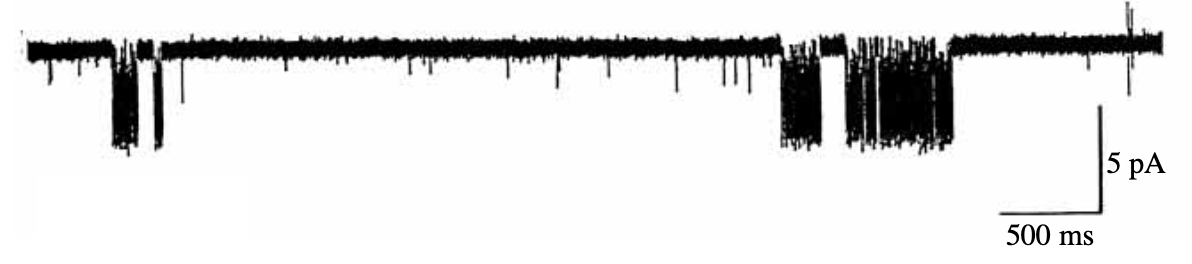
\includegraphics[width=.8\textwidth]{Patch_clamp_current_records.png}
\caption{Typical current record from a single channel patch clamp experiment.}
\label{fig:patch_single_ch}
\end{figure}

\section{Minchie}



\begin{figure}
\centering
\subfloat[]{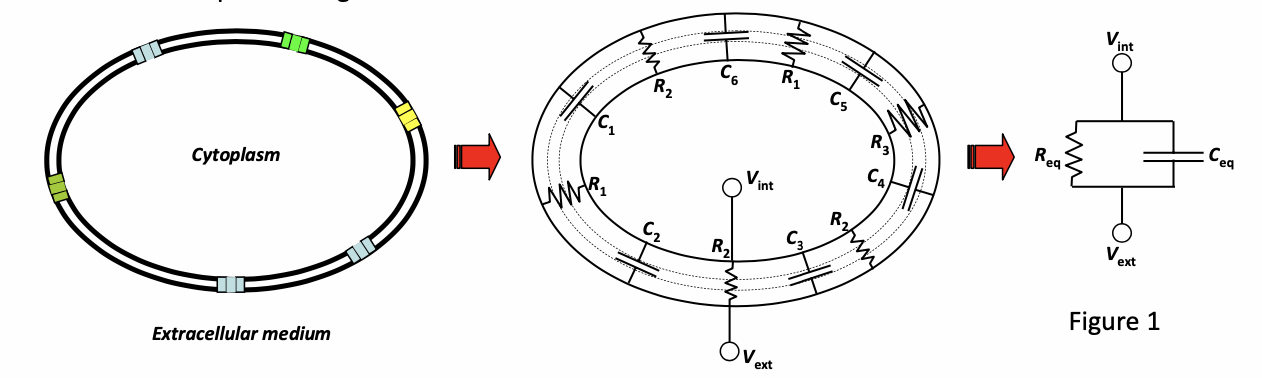
\includegraphics[width=.7\textwidth]{Cell_scheme_derivation.png}\label{fig:cell_scheme_derivation}}
\subfloat[]{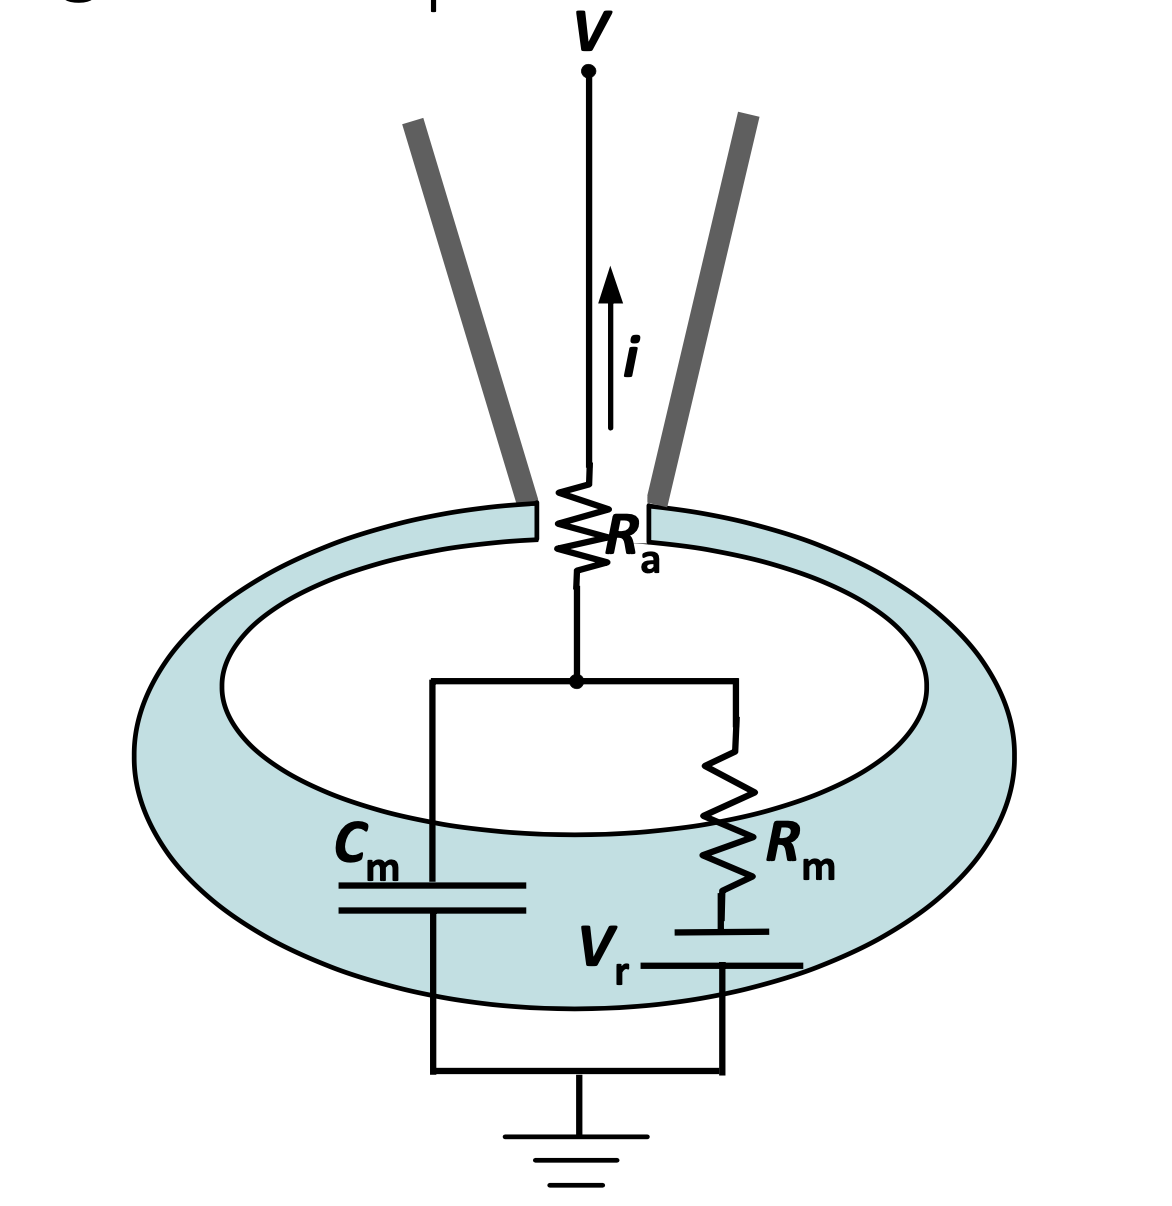
\includegraphics[width=.29\textwidth]{Cell_scheme.png}\label{fig:cell_scheme}}
\caption{\textbf{(a)} Derivation of the electrical scheme for a cell; \textbf{(b)} Schematic representation of the electrical properties of a cell}

\end{figure}

The simulation performed in this exercise is aimed to discover the response of a cell in a whole cell patch clamp configuration to a square wave electrical stimulus.

In order to get meaningful predictions on the behavior of the cell one must summarize the electrical properties of the system in an electrical scheme, namely the one in figure \ref{fig:cell_scheme}.
As a first approximation, one can consider the cell membrane as made of a lipid bilayer and ion channels, which can be electrically schematized by capacitors and resistances.
The fact that both these components experience the same potentials at the two sides, leads us to the conclusion that they must be connected in parallel we will indicate the total capacity and resistance of the cell membrane with $C_m$ and $R_m.$
As in this exercise we are considering whole cell patch clamp configuration, access resistance $(R_a)$ of the pipette must be considered as well; the voltage applied is controlled by the experimenter by setting the pipette potential: we will indicate this value with $V.$

In the following passages we will derivate the equations that link the electrical parameters of the simulation $C_m, R_m, R_a$ and $V$ to the current $i$ flowing through the cell.

The system is described by the first order linear differential equation derived from Kirchoff laws:
\begin{equation}
    \tau\dv{V_m}{t} = -V_m +V \frac{R_m}{R_m+R_a} \qq{with} \tau = \frac{R_a R_m}{R_a + R_m}C_m,
    \label{eq:update_vm}
\end{equation}
where $V_m$ is the membrane potential as defined above.
The current flowing through the membrane in the small time interval $[t,t+\dd{t}]$ can be computed as 
\begin{equation}
i(t+\dd{t}) = \frac{V_m(t)}{R_m} + C_m \dv{V_m}{t} {(t)}
\label{eq:update_current}
\end{equation}
A numerical solution for the behavior of the current signal in time is obtained with time discretization and the implementation of \eqref{eq:update_current} and \eqref{eq:update_vm} as update rules at each step.
In pseudo-code using $j$ as time index it results in:
\begin{equation}
    \begin{cases}
        \dv{V_m}{t} = -V_m(j) + V_{in}(j)\frac{R_m}{\tau(R_m +R_a)}\\
        i(j)= \frac{Vm(j)}{R_m} +C_m \dv{V_m}{t}\\
        Vm(j+1) = V_m(j) +\dd{V_m} \dd{t}
    \end{cases}
\end{equation}
Note that in this expression we set $V_{in}$ as a time dependent quantity: this is motivated by the fact that we want to simulate the behavior of the pipette-cell system for an input voltage that has the shape of a square wave.

The result of such numeric process is the numerical estimation of the behavior of the current as a function of time.
This output, as depicted with a red line in figure \ref{mah}, is a smooth function of time.
However in real laboratory situations noise come into play, modifying the ideal shape of the signal from a smooth curve to a disturbed one.
Therefore, in order to produce a more realistic simulation, noise has been added to the signal (blue line in figure \ref{mah}).
The distribution of the noise of the signal is non trivial and could in principle depend on many factors, such as cell parameters like membrane resistance or capacitance, ambient parameters like temperature or even on factors related to the experimental apparatus itself.
In this work I chose to assign Gaussian distribution to noise for simplicity; I set the amplitude of this noise in order to make the signal resemble the example shown in class during the discussion of Patch Clamp experiments.

In a laboratory situation we would be interested in retrieving the experimental parameters from data, namely $\tilde{R}_a, \tilde{R}_m$ and $\tilde{C}_m.$
To perform this task we are helped by the analytical solution for current of the system described above in the case of a square wave of amplitude $V$:
\begin{equation}
     i(t)=\frac{V\pqty{1+\frac{R_a}{R_m}}}{R_a+R_m} e^{-\frac{t-t_0}{\tau}}
 \end{equation} 
which is equal to:
\begin{equation}
i(t)=
    \begin{cases}
        \frac{V}{R_a} &\text{ if }t=t_0\\
        \frac{V}{R_a + R_m} &\text{ if } t>>\tau.
        
    \end{cases}
\end{equation}
Starting from this expression and calling $i(t=t_0)=i_{pk}$ and $i(t>>\tau) = i_\infty$ one can use these two current values to retrieve:
\begin{equation}
    \tilde{R}_a= \frac{V}{i_{pk}}\qq{and}\tilde{R}_m = \frac{V}{i_\infty} - R_a
    \label{eq:Ra_estimation}
\end{equation}
Finally, the estimation of $C_m$ is done using \eqref{eq:update_vm} and the experimental value of $\tau:$
\begin{equation}
    \tilde{C}_m = \tilde{\tau}\pqty{\frac{1}{\tilde{R}_a}+\frac{1}{\tilde{R}_m}}.
\end{equation}

Similar equations hold also when the cell presents a resting potential, namely if we call it $V_r$ the analytical solution becomes: 
\begin{equation}
    i(t) = i_\infty + \frac{V \frac{R_a}{R_m} e^{-\frac{t-t_0}{\tau}}}{R_a+R_m}\qq{with} i_\infty= \frac{V-V_r}{R_a+R_m}
\end{equation}
and the equations for the experimental parameters become:
\begin{align}
&\hat{R}_a = \bqty{\frac{i_{pk}-i_\infty}{V} + \frac{i_\infty}{V-V_r}}^{-1}\\
&\hat{R}_m = \frac{V-V_r}{i_\infty} - \hat{R}_a\\
&\hat{C}_m = \tau\pqty{\frac{1}{\hat{R}_a}+\frac{1}{\hat{R}_m}}
\end{align}


The final part of the simulation involved, as in real experiments, the presence of a 4-pole low pass Bessel filter aimed to "clean" the signal from high-frequency noise.
As will be discussed later, the presence of this component effectively reduce the HF signal noise over the threshold frequency, however a side effect is introduced: signal peaks are shifted in time and lowered in magnitude.
This behavior is particularly bad for our estimation, since the derivation of the access resistance is performed starting from the peak value of the current (see \eqref{eq:Ra_estimation}) that is no more accurately reported by the experimental setup.

To overcome this problem, another method can be used to esteem the experimental value of the access resistance $\tilde{R}_a.$
Starting from equation \eqref{eq:update_vm} and its solution for voltage, namely
\begin{equation}
    V_m(t) = \frac{V R_m}{R_a+R_m} \pqty{1-e^{-t/\tau}}
\end{equation}
one can express the current flowing through $R_a$ as the sum of a regime current and a transient current
\begin{equation}
    i_{R_a} = i_{C_m} + i_{R_m} = i_{tr}+ i_\infty \qq{with} i_{tr} = Ae^{-t/\tau}, \quad A \text{ constant.}
    \label{eq:current_transient}
\end{equation}
The total charge transfered from transient current is given by:
\begin{equation}
    Q_{tr} = \int_0^\infty Ae^{-t/\tau}\dd{t} = \frac{i_{tr}}{\tau}
\end{equation}
therefore, substituting in \eqref{eq:current_transient} we get
\begin{equation}
    i_{R_a} = \frac{Q_{tr}}{\tau} + i_\infty
\end{equation}
and finally
\begin{equation}
    \tilde{R}_a = \frac{V}{i_{R_a}} = \frac{\tau V}{Q_{tr} + \tau i_\infty}.
\end{equation}
This procedure can be implemented in the offline digital analysis by numerically integrating the signal to get the transferred charge and then retrieve the experimental value for the access resistance.

\section{Results, finally! :-)}
\begin{figure}
\centering
\subfloat[]{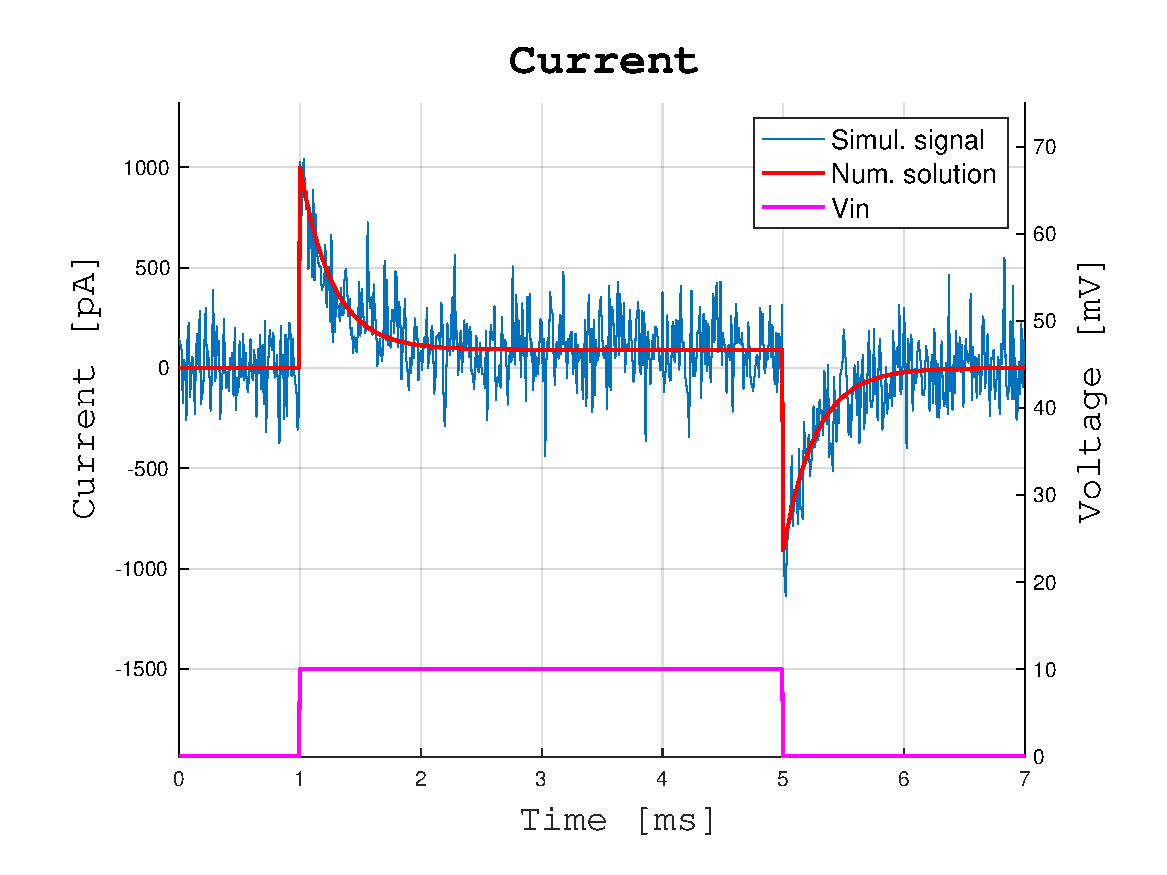
\includegraphics[width=.49\textwidth]{Current.pdf}\label{fig:current}}
\subfloat[]{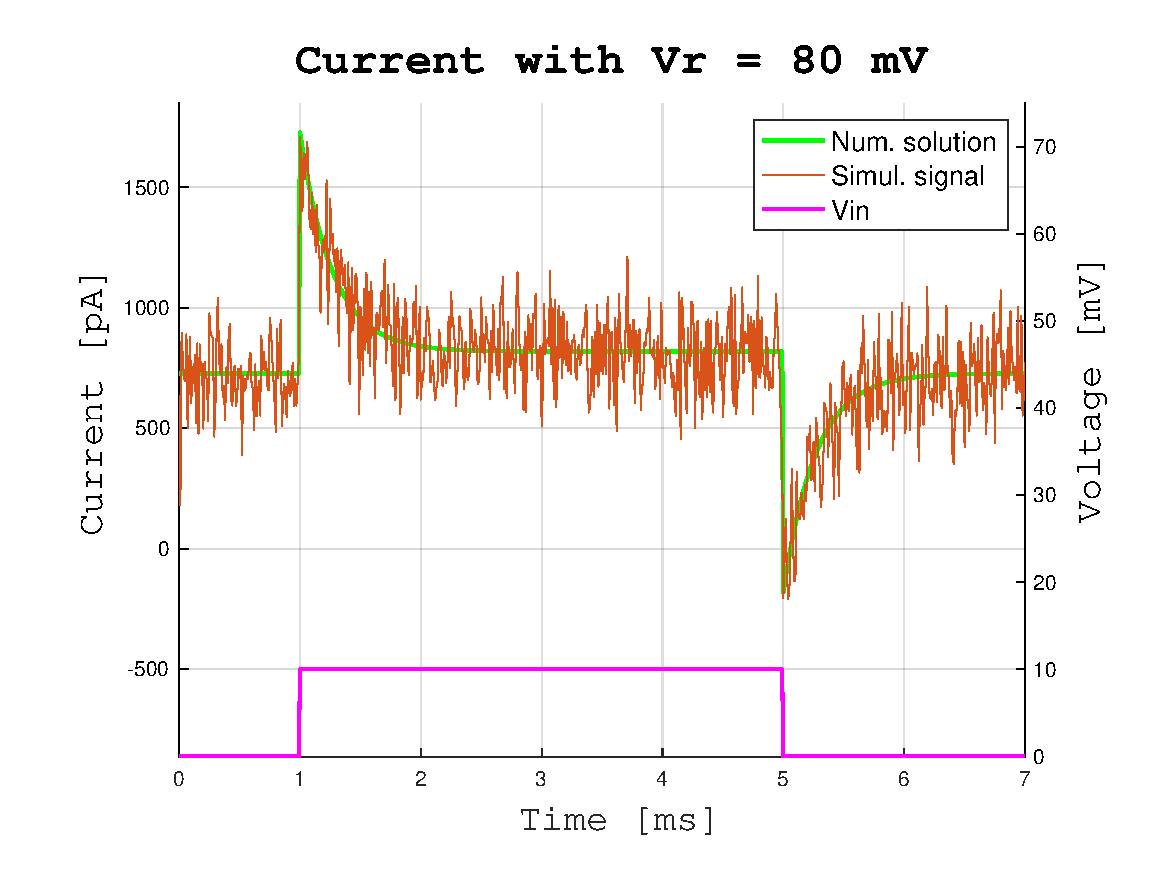
\includegraphics[width=.49\textwidth]{Current_r.pdf}\label{fig:current_r}}
\caption{\textbf{(a):} Current signal; \textbf{(b):} current signal with 80 mV resting potential}
\end{figure}

\begin{table}[h]
\caption{Experimental parameters retrieved from simulation, unfiltered signal}
\label{tab:parameters_nofilter}
\vspace{-.4cm}
\centering
\[
\begin{array}{cccc}
\toprule
\bm{V_r}\ [\si{\mV}]&\bm{\tilde{R}_a}\ [\si{\mega \ohm}]&\bm{\tilde{R}_m}\ [\si{\mega\ohm}]& \bm{\tilde{C}_m}\ [\si{\pico\farad}]\\
\midrule
0&11.1\pm 0.7& 107.4 \pm 11 & 26\pm 5\\
80 & 12.6\pm 0.5 & 96\pm11 & 22\pm 5\\ 
\bottomrule
\end{array}
\]
\end{table}

\begin{figure}
\centering
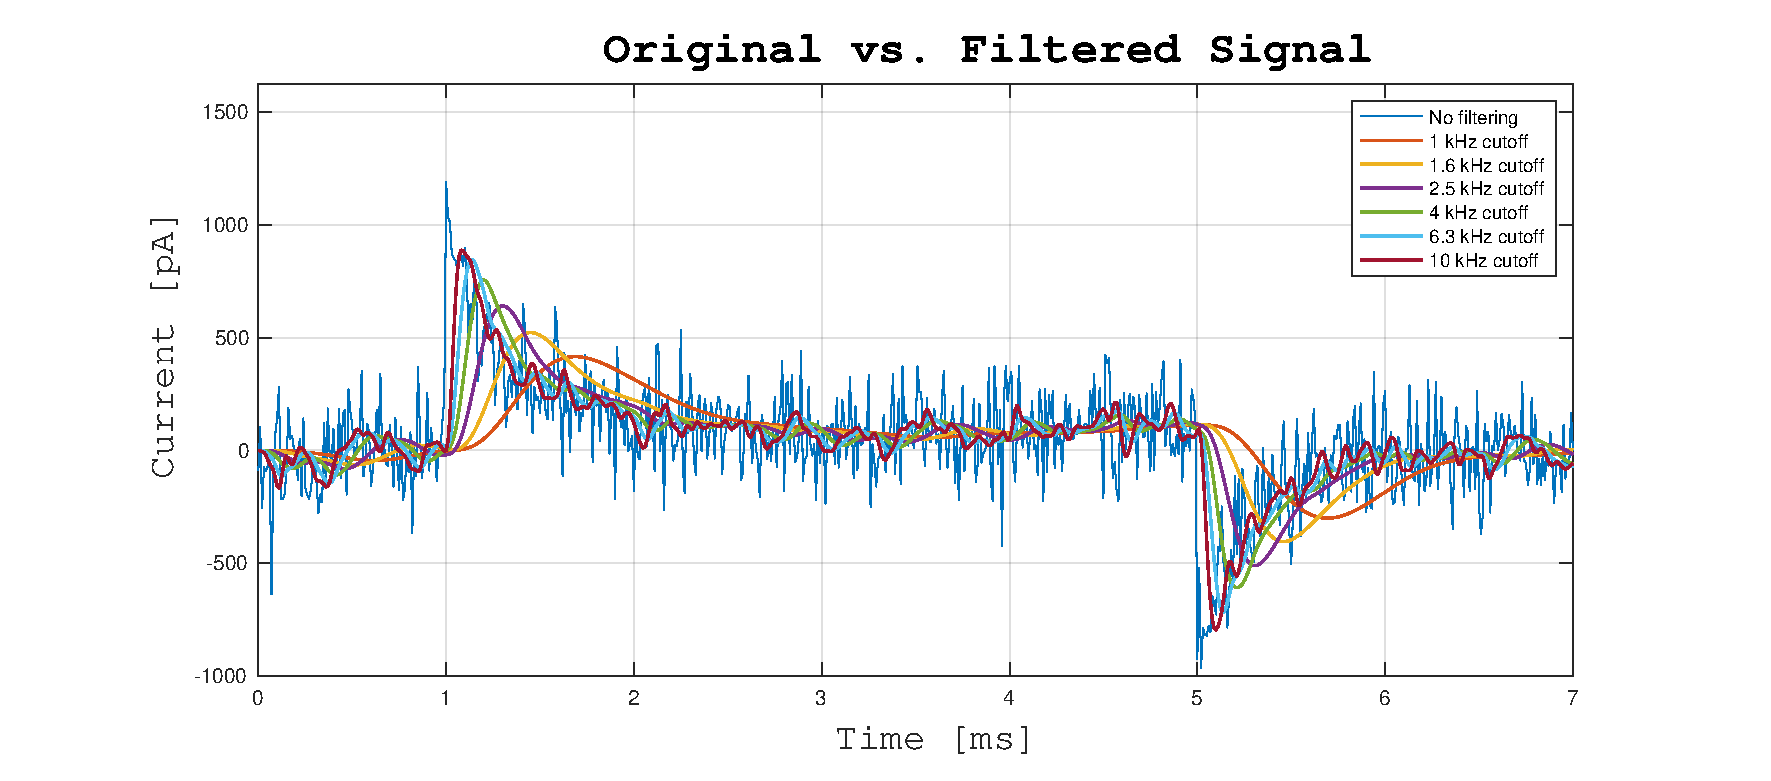
\includegraphics[height=6.5cm]{Bess_all_freq.pdf}
\caption{Comparison between original noisy signal and filtered signals at various cutoff frequencies}
\label{fig:Bess_all_freq}
\end{figure}

\begin{figure}
\subfloat{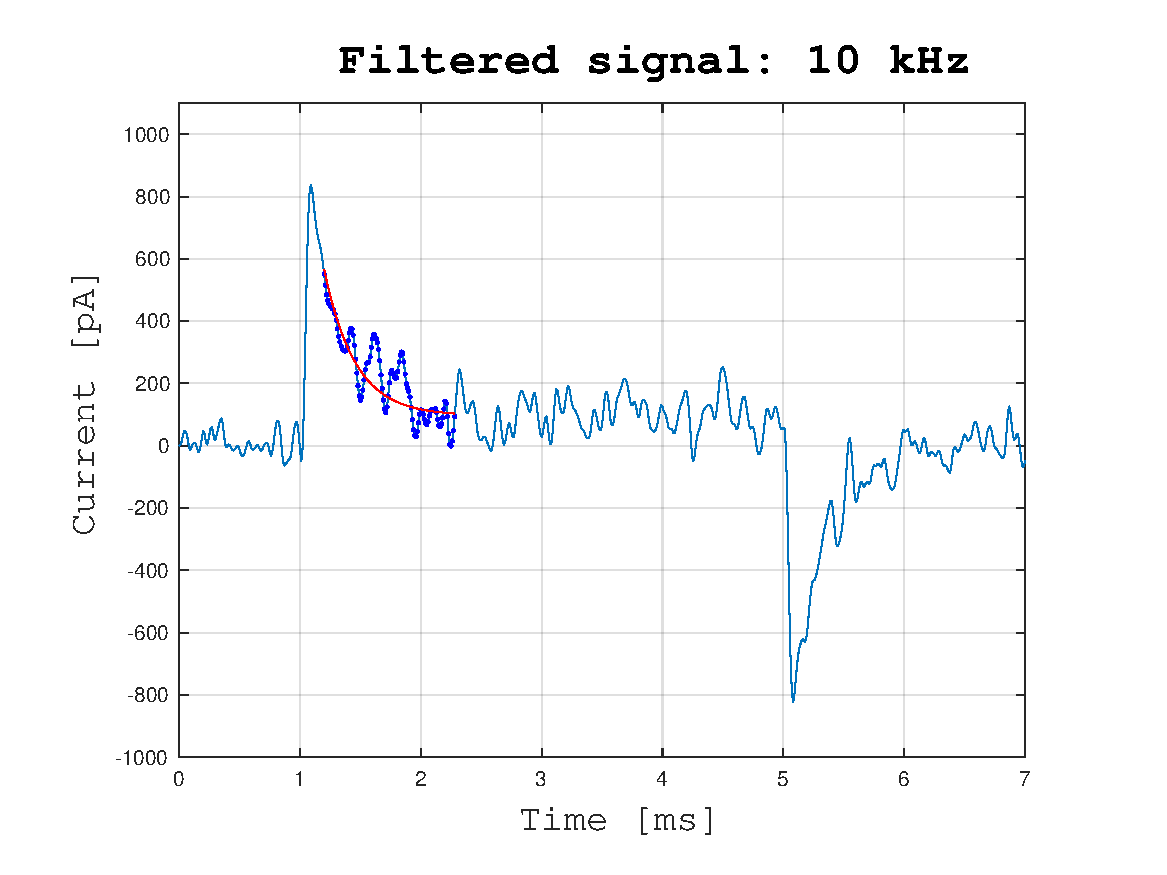
\includegraphics[width=.48\textwidth]{Bess10000Hz.pdf}\label{fig:bess10k}}
\subfloat{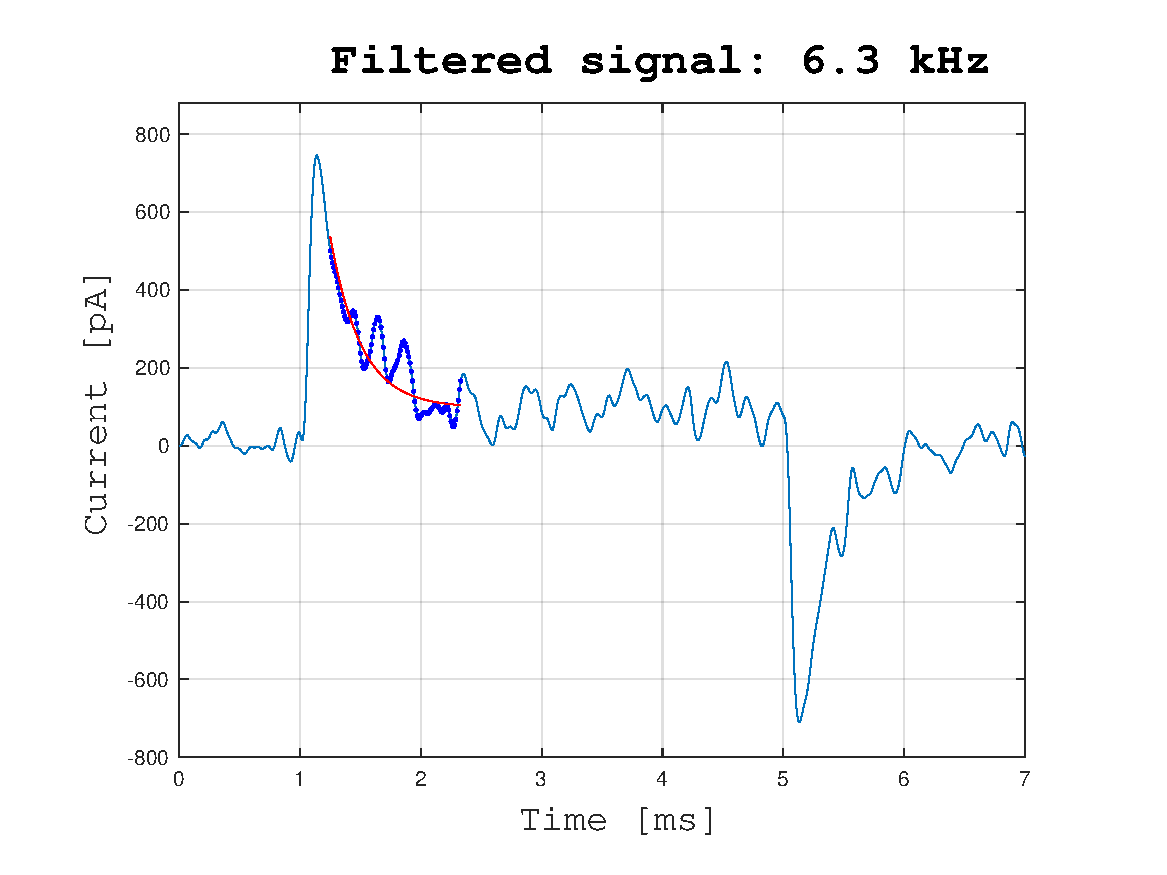
\includegraphics[width=.48\textwidth]{Bess6310Hz.pdf}\label{fig:bess6_3k}}

\subfloat{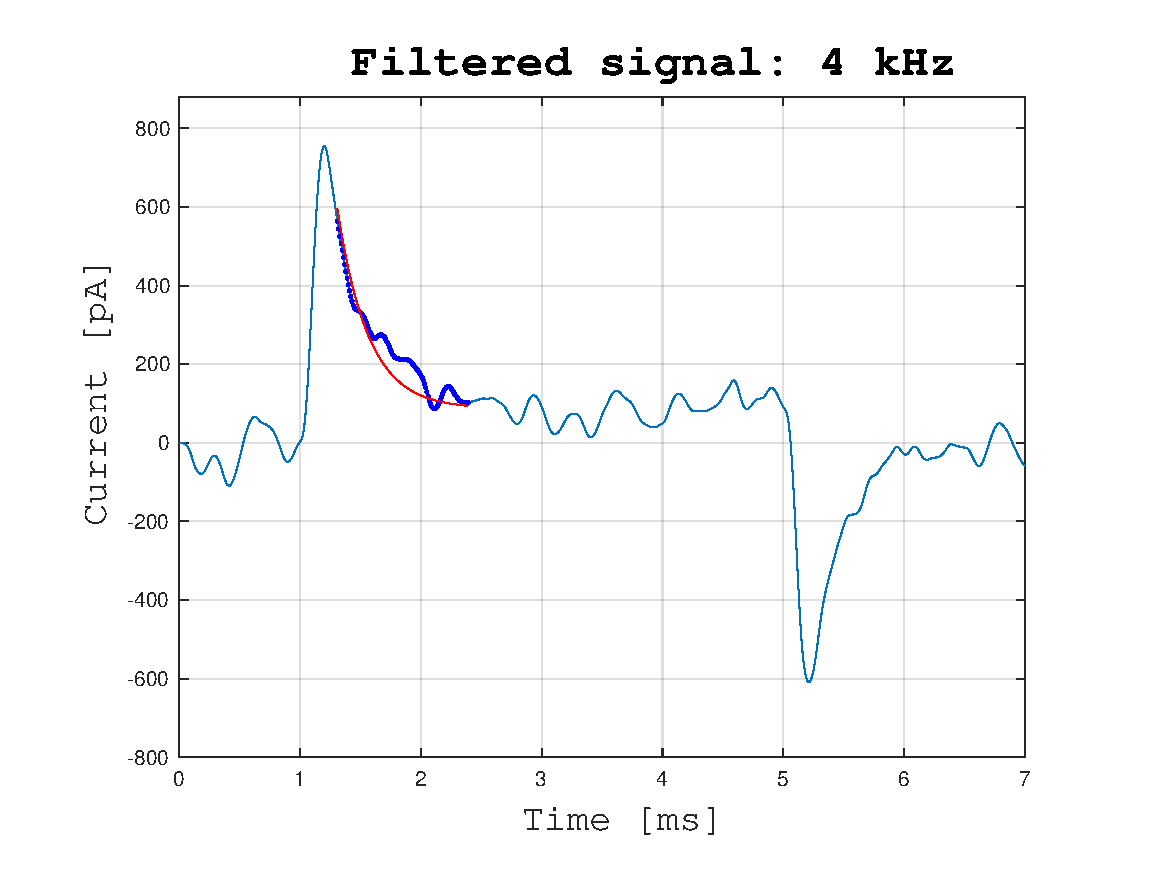
\includegraphics[width=.48\textwidth]{Bess3982Hz.pdf}\label{fig:bess4k}}
\subfloat{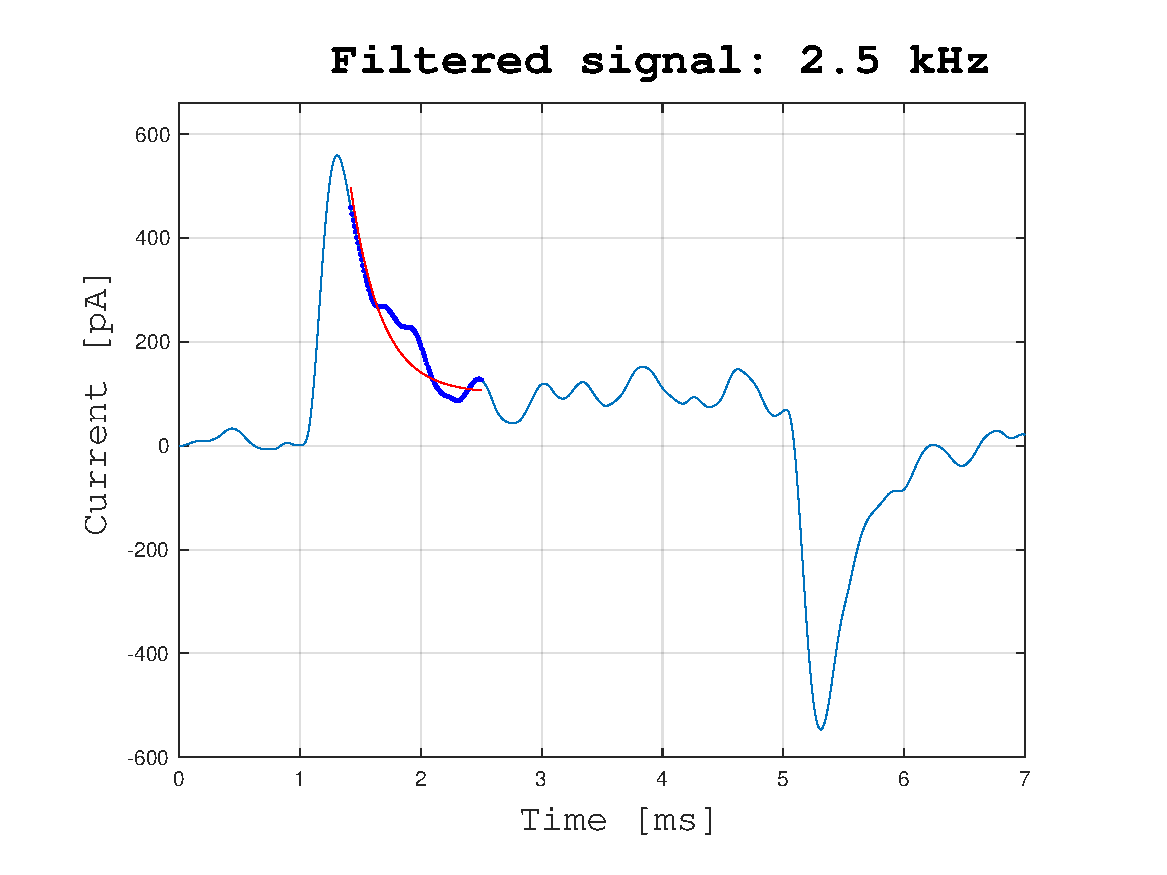
\includegraphics[width=.48\textwidth]{Bess2512Hz.pdf}\label{fig:bess2_5k}}

\subfloat{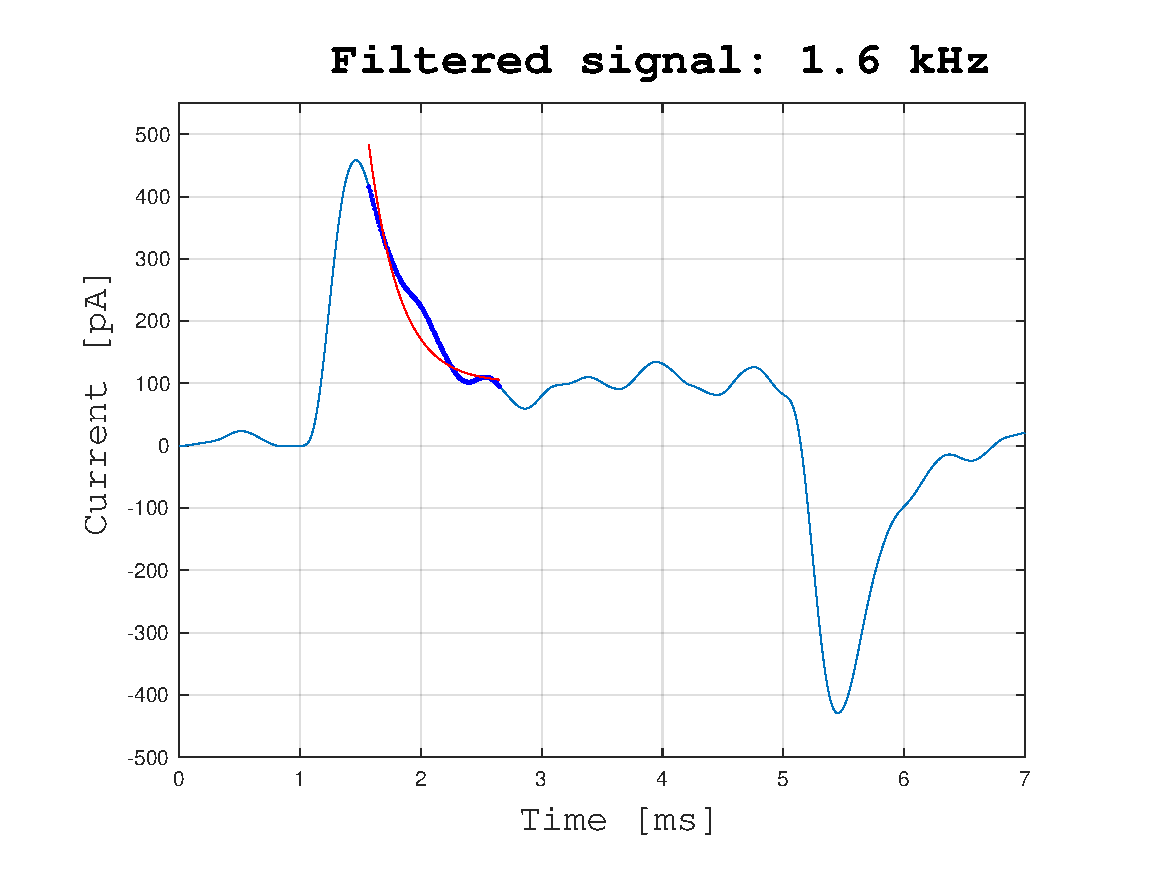
\includegraphics[width=.48\textwidth]{Bess1585Hz.pdf}\label{fig:bess1_5k}}
\subfloat{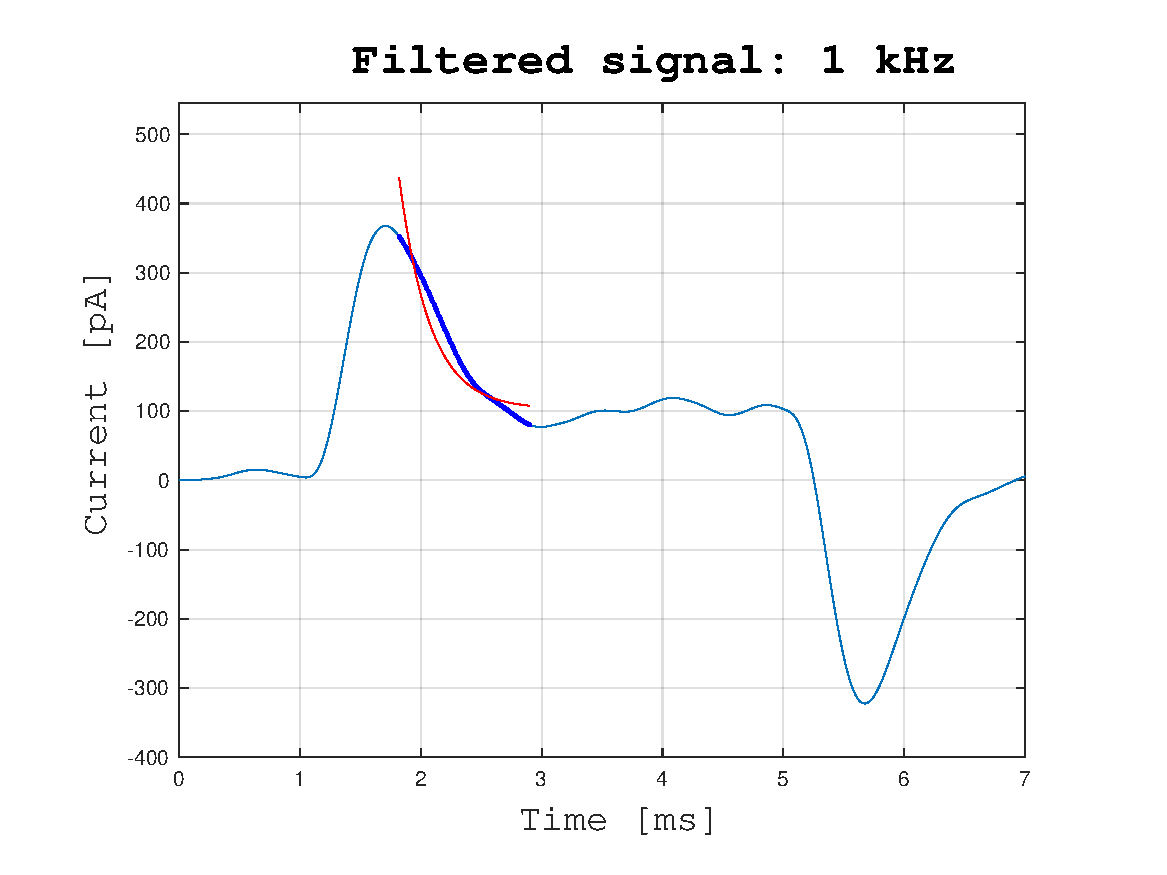
\includegraphics[width=.48\textwidth]{Bess1000Hz.pdf}\label{fig:bess1k}}

\caption{Filtered signals at various cutoff frequencies, namely: 10, 6.3, 4, 3, 2.5, 1.6 and 1 kHz}
\label{fig:current_filtered}
\end{figure}


\begin{table}[h]
\caption{Experimental parameters retrieved from simulation, filtered signals}
\label{tab:parameters_nofilter}
\vspace{-.4cm}
\centering
\[
\begin{array}{cccc}
\toprule
\textbf{Cutoff}\ [\si{\hertz}]&\bm{\tilde{R}_a}\ [\si{\mega \ohm}]&\bm{\tilde{R}_m}\ [\si{\mega\ohm}]& \bm{\tilde{C}_m}\ [\si{\pico\farad}]\\
\midrule
1000    &   21.5    \pm 0.7 &   83  \pm 1   &   14.9    \pm 0.6 \\
1585    &   14  \pm 1   &   90  \pm 2   &   22  \pm 3   \\
2512    &   12  \pm 1   &   91  \pm 2   &   24  \pm 4   \\
3981    &   12  \pm 1   &   91  \pm 2   &   25  \pm 4   \\
6310    &   11  \pm 2   &   93  \pm 3   &   25  \pm 5   \\
10000   &   11  \pm 2   &   95  \pm 4   &   25  \pm 5   \\
\bottomrule
\end{array}
\]
\end{table}




















\end{document}
